\section{Katz/Kelley comparison}
\begin{figure}[H]
%/data/ap4909/30.10.2013-hot_cold_geochem/sample_testing/southern_marianas/kelley/mf_vs_ti.py
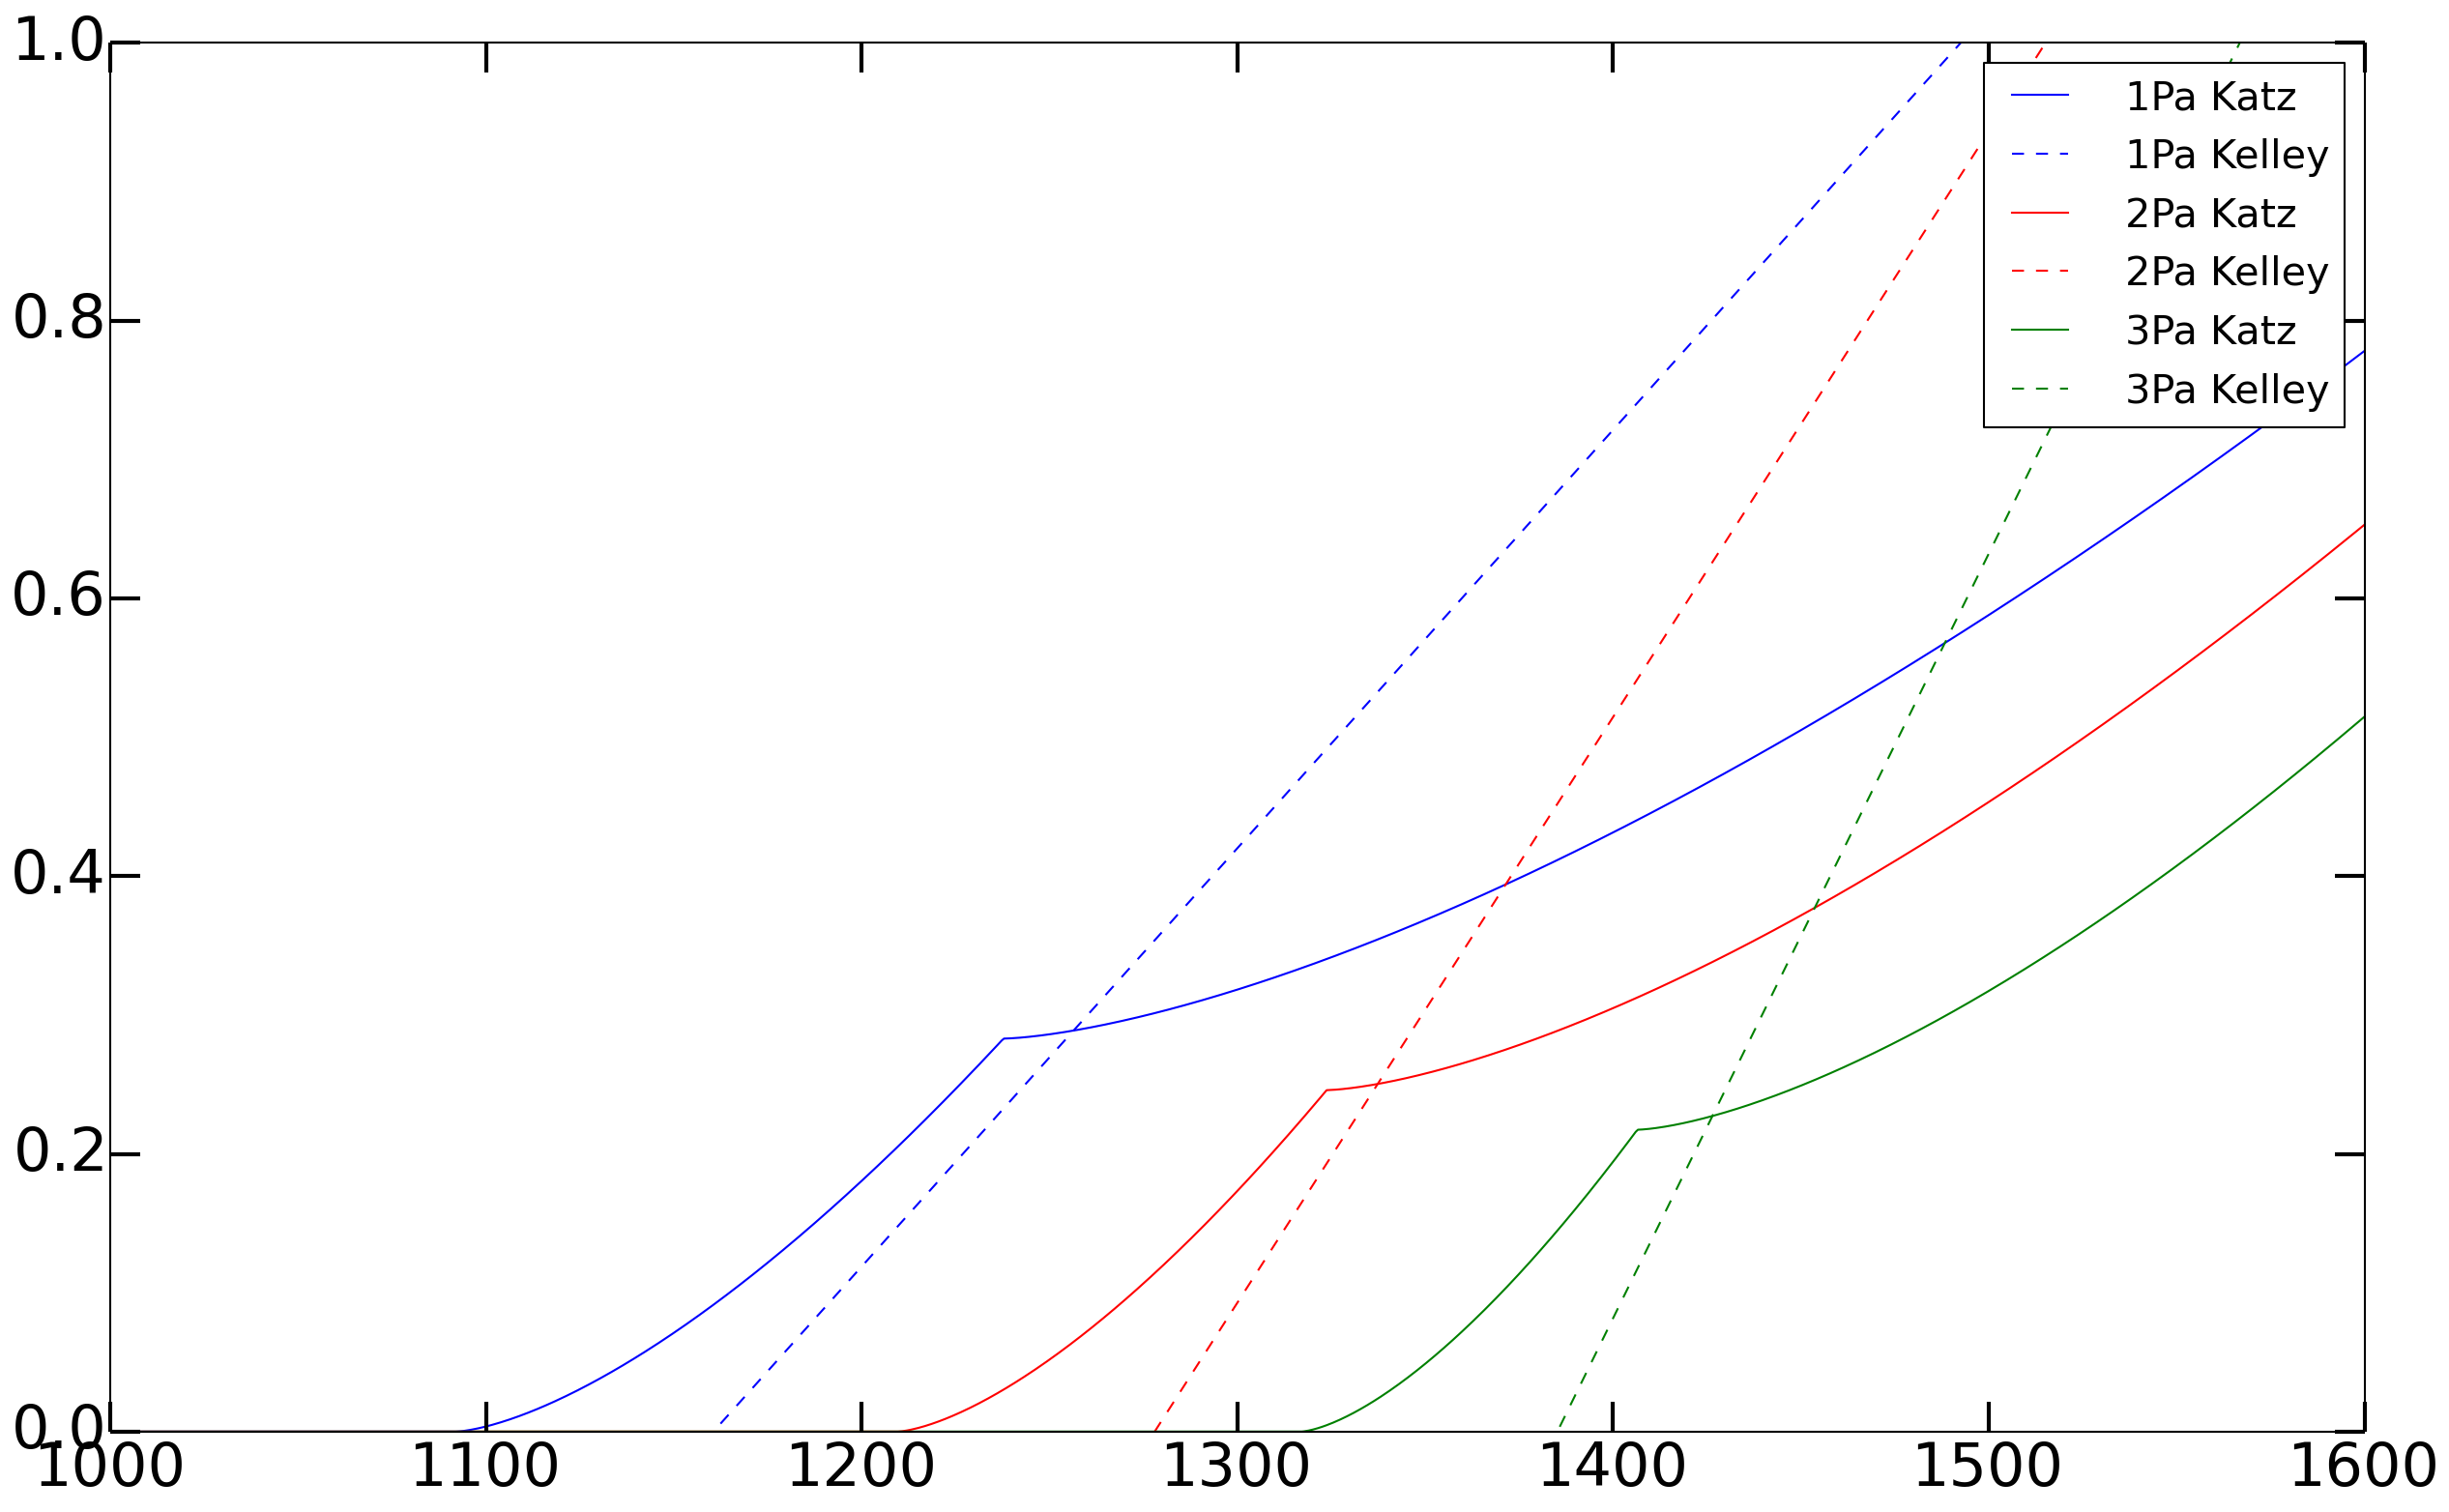
\includegraphics[width=0.9\textwidth]{/data/ap4909/30.10.2013-hot_cold_geochem/sample_testing/southern_marianas/kelley/kelley_katz_comparison/figures/katz_kelley_comparison.png}
\label{ti_resid_v_f}
\captionsetup{singlelinecheck=off}
\caption[]{
\begin{itemize}
\item Assuming 4 wt\% H2O for our samples, 0.25 fo2. 
\end{itemize}
}
\end{figure}

\begin{figure}[H]
%/data/ap4909/30.10.2013-hot_cold_geochem/sample_testing/southern_marianas/kelley/mf_vs_ti.py
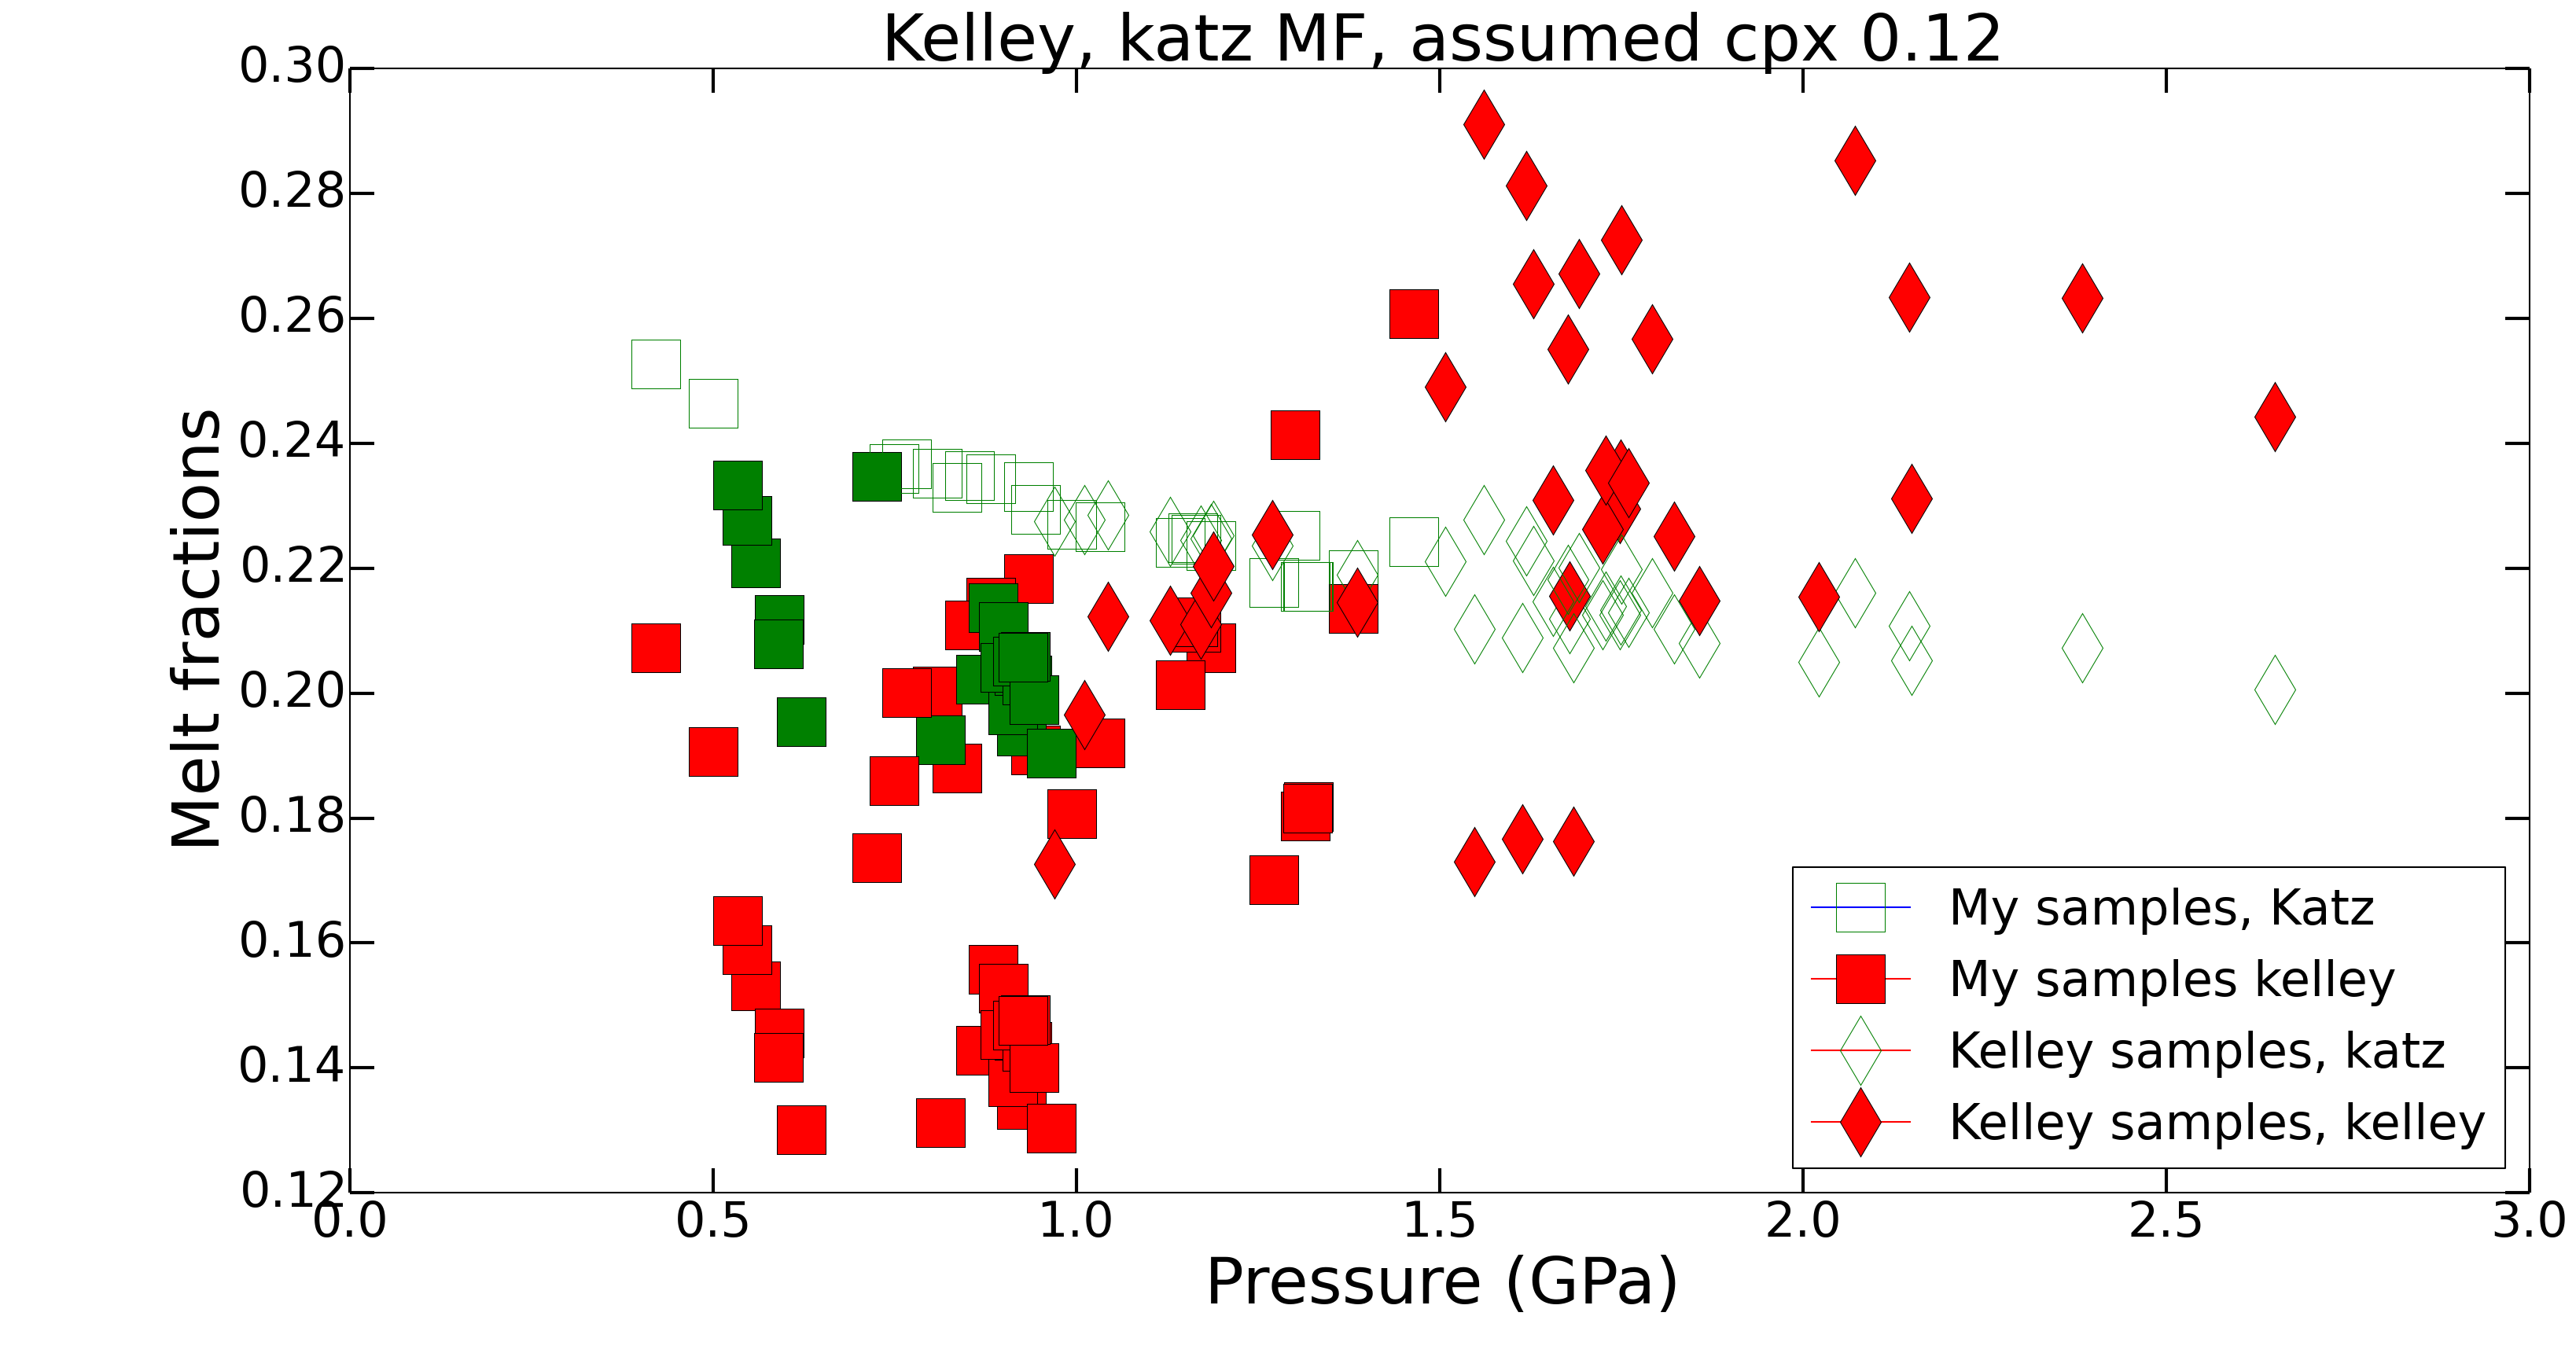
\includegraphics[width=0.9\textwidth]{/data/ap4909/30.10.2013-hot_cold_geochem/sample_testing/southern_marianas/kelley/kelley_katz_comparison/figures/melt_fractions/katz_kelley_mf_vs_P.png}
\label{ti_resid_v_f}
\captionsetup{singlelinecheck=off}
\caption[]{
\begin{itemize}
\item Assuming 4 wt\% H2O for all samples, 0.25 fo2. 

\item hollow symbols - cpx has been exhausted.
\item Below 1GPa Katz MF higher than Kelley MF - due to lower solidus of Katz.
\item Above 1 GPa - Kelley do not consider cpx out - generally higher melt fractions.
\item With increasing pressure, a certain cpx content can be exhausted quicker - this effect is incorporated with Katz, and is why more samples exhaust CPX at increasing pressure.
\item Kelley also have a dT/dF variation with pressure, leading to higher melt productivities at higher pressures.

\end{itemize}
}
\end{figure}
\begin{figure}[H]
%/data/ap4909/30.10.2013-hot_cold_geochem/sample_testing/southern_marianas/kelley/mf_vs_ti.py
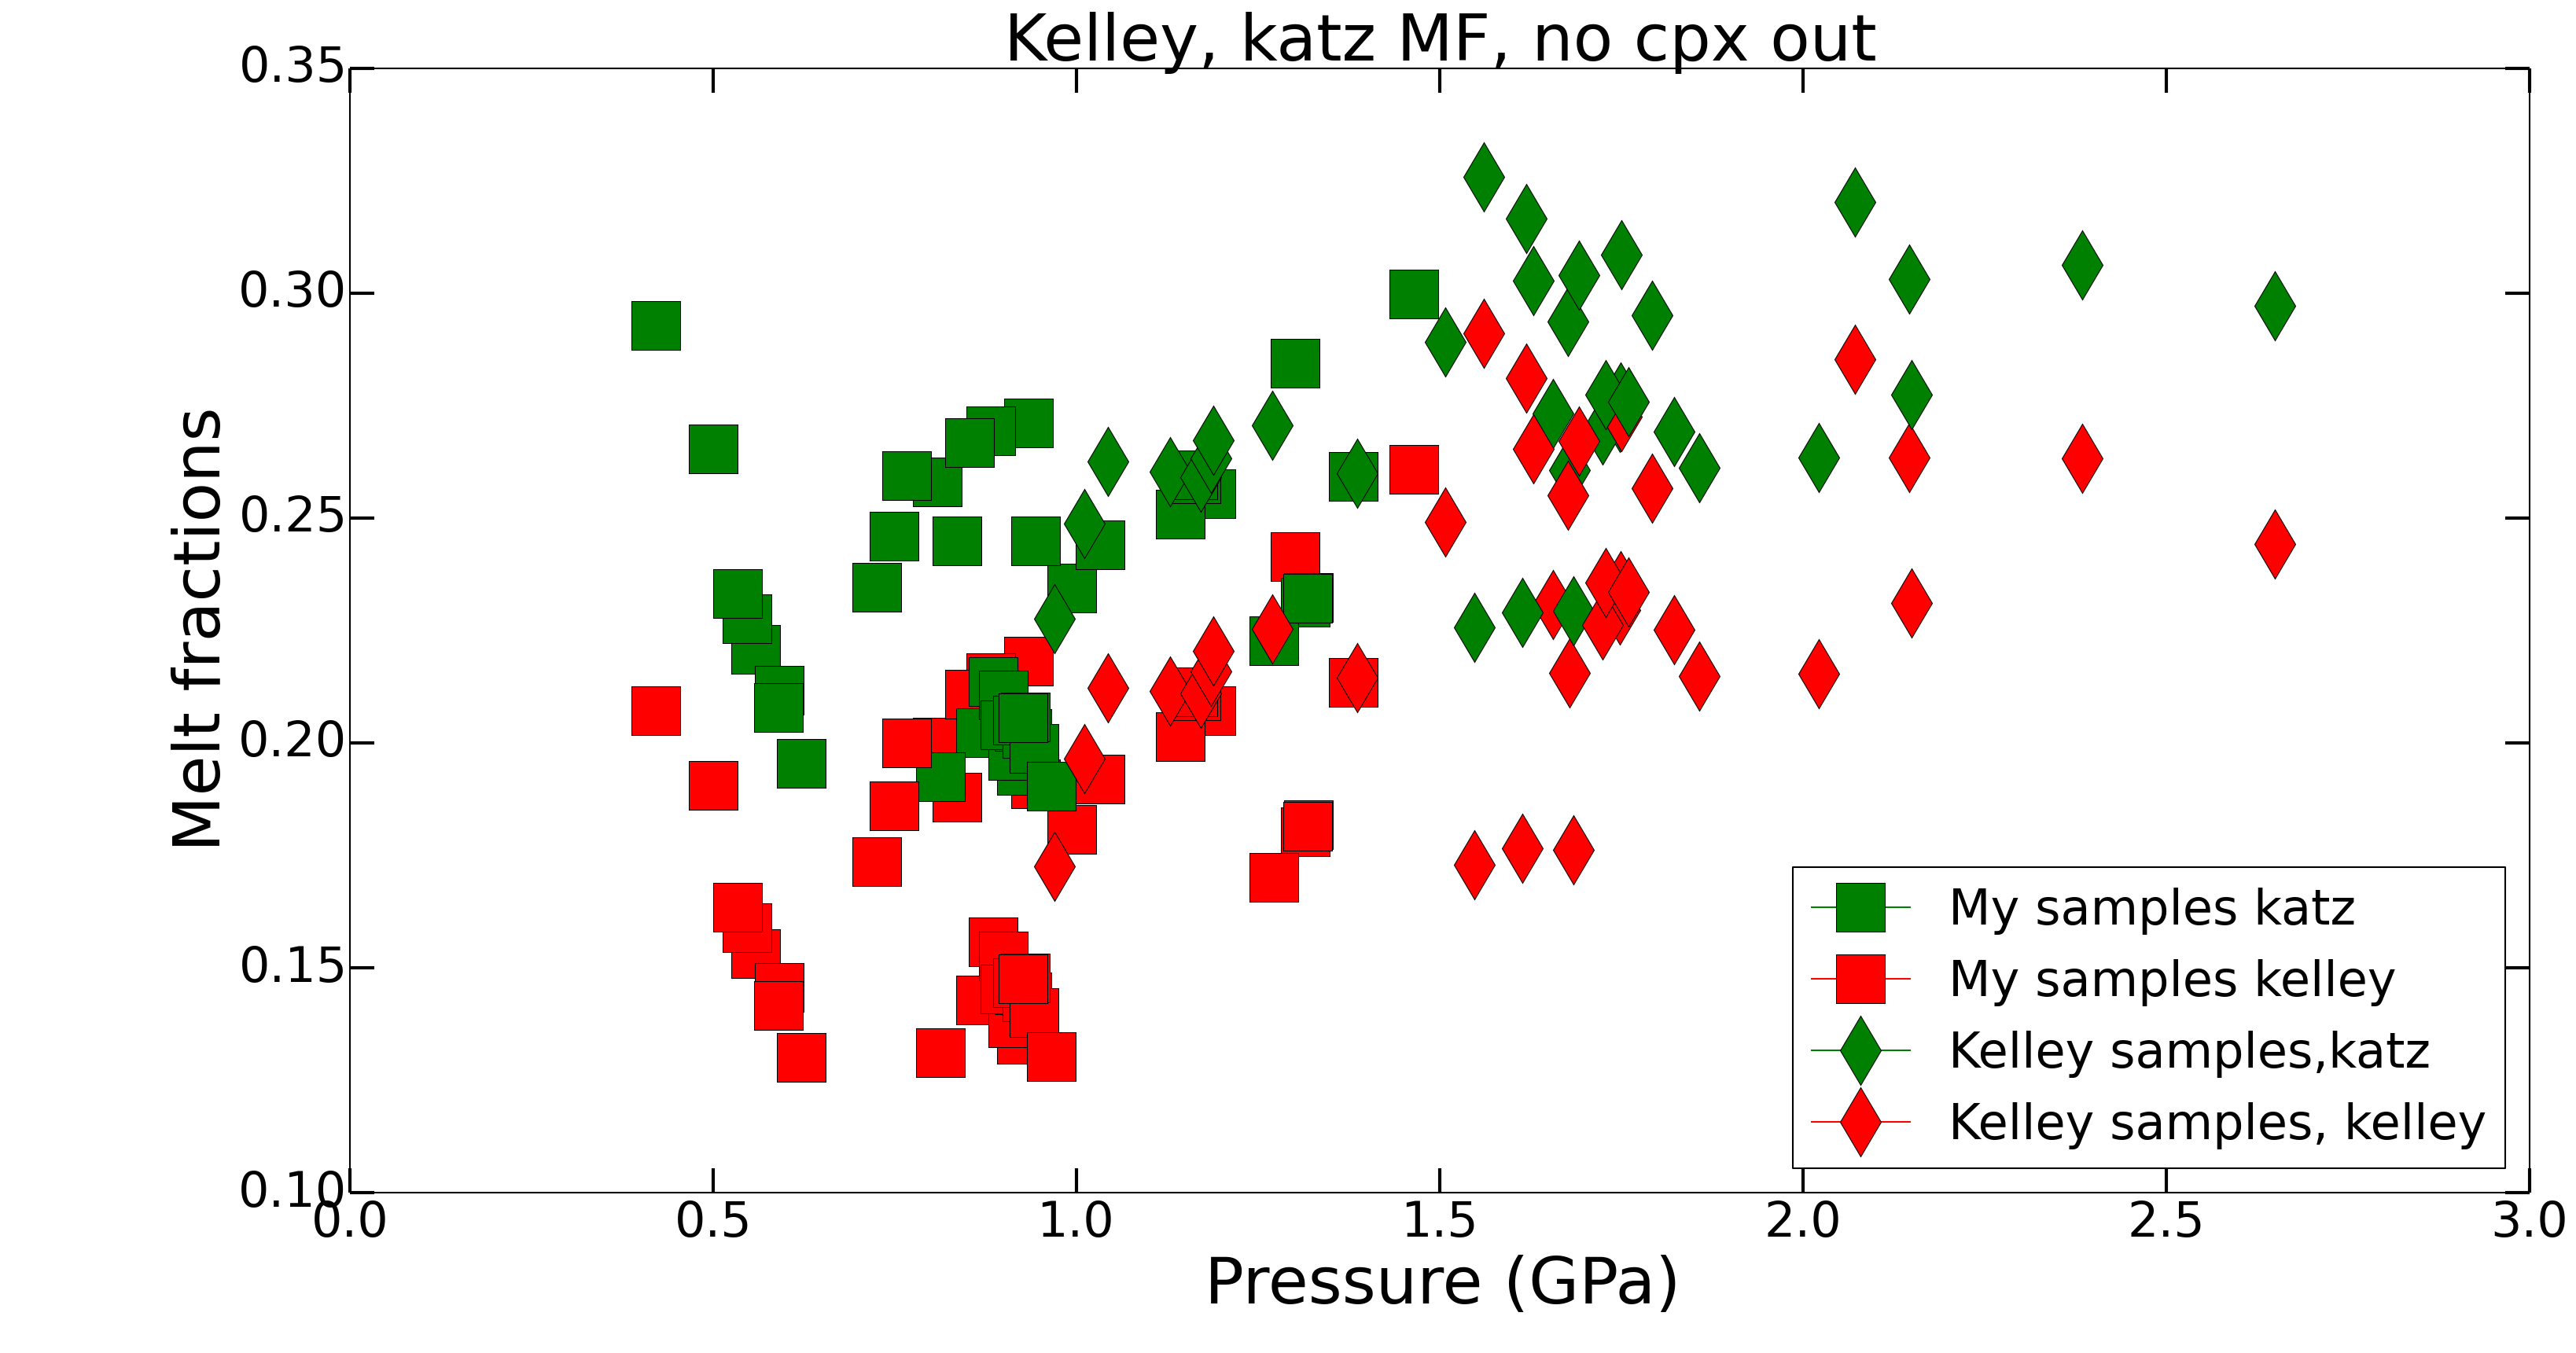
\includegraphics[width=0.9\textwidth]{/data/ap4909/30.10.2013-hot_cold_geochem/sample_testing/southern_marianas/kelley/kelley_katz_comparison/figures/melt_fractions/katz_kelley_mf_vs_P_no_katz_cpx_out.png}
\label{ti_resid_v_f}
\captionsetup{singlelinecheck=off}
\caption[]{
\begin{itemize}
\item Assuming 4 wt\% H2O for all samples, 0.25 fo2. 
\item When cpx exhaustion is excluded from Katz calculation, 
\end{itemize}
}
\end{figure}
\begin{figure}[H]
%/data/ap4909/30.10.2013-hot_cold_geochem/sample_testing/southern_marianas/kelley/mf_vs_ti.py
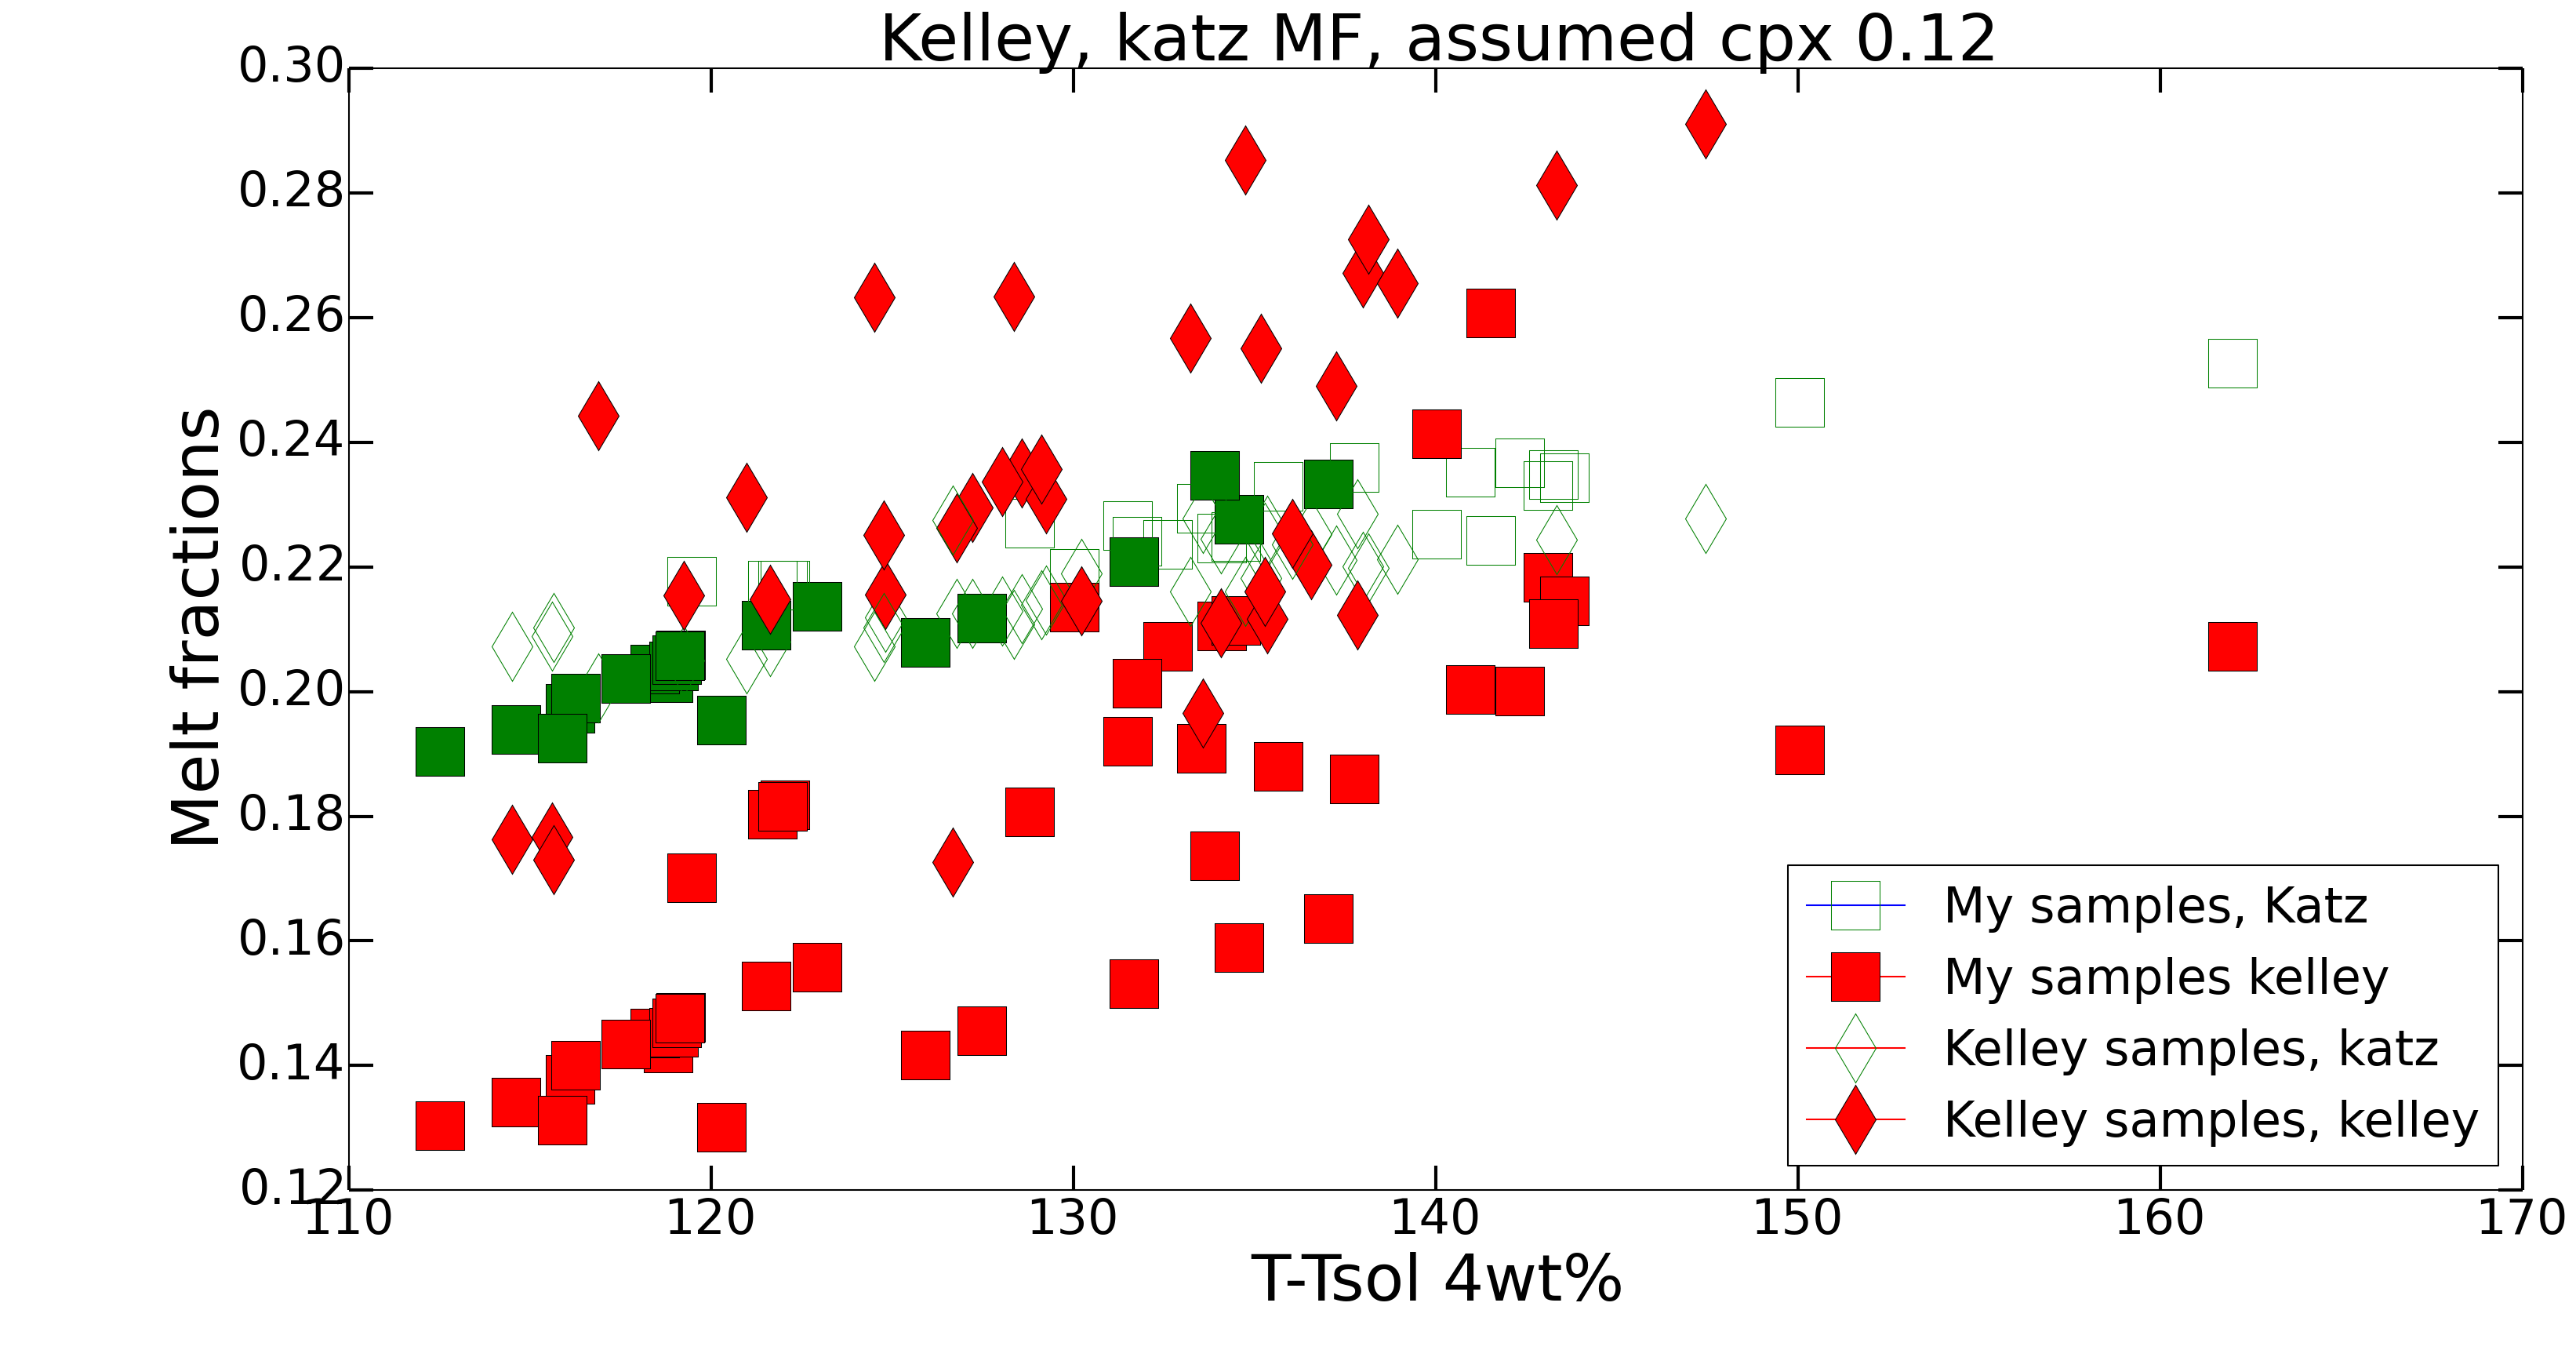
\includegraphics[width=0.9\textwidth]{/data/ap4909/30.10.2013-hot_cold_geochem/sample_testing/southern_marianas/kelley/kelley_katz_comparison/figures/melt_fractions/katz_kelley_mf_vs_t_minus_tsol.png}
\label{ti_resid_v_f}
\captionsetup{singlelinecheck=off}
\caption[]{
\begin{itemize}
\item Assuming 4 wt\% H2O for all samples, 0.25 fo2. 
\item When cpx exhaustion is excluded from Katz calculation, 
\end{itemize}
}
\end{figure}

